\begin{figure}[h!]
	\begin{center}
		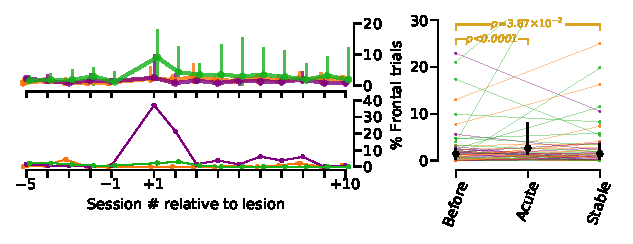
\includegraphics[scale=1]{ch-appendicies/figures/FrontalTrials.pdf}
		\caption[Frontal Trials After Striatal Lesion]
		{\textbf{Dorsal striatum lesions induced a transient increase in the percentage of trials during which animals remained close to the reward area.}
		\textit{Upper left}: Session-by-session percentage of trials in which animals remained close to the reward area (i.e., frontal trials).
		Group data for animals with DLS, DMS and DS lesion.
		Same color code for lesion types as in \autoref{fig:lesion:task}.
		\textit{Lower left}: Same as above, but for the illustrative animals, shown in \Autoref{fig:lesion:task}{E-G}.
		\textit{Right}: Group statistical comparisons before and after striatal lesion.
		There is an acute increase that is mostly restored after a few sessions.		
		}
		\label{fig:appendix:Frontal}
	\end{center}
\end{figure}